\documentclass{article}
\usepackage[T1]{fontenc}
\usepackage{lmodern}
\usepackage{graphicx}
\usepackage{amsmath,amssymb}
\usepackage[a4paper,margin=2cm]{geometry}
\usepackage[absolute,overlay]{textpos}
\setlength{\TPHorizModule}{1mm}
\setlength{\TPVertModule}{1mm}
\usepackage[indonesian]{babel}
\usepackage{hyperref}
\setlength{\emergencystretch}{2em}
% unit: Halaman 5

\begin{document}

% === Halaman 5 (llm) ===

\begin{itemize}
  \item Contoh: \[ y^2 = x^3 - 4x \\ = x(x-2)(x+2) \]
\end{itemize}

\vspace{80mm}

\textcolor{red}{Sumber gambar: Andreas Steffen, Elliptic Curve Cryptography}

% deskripsi: Grafik kurva eliptik y^2 = x^3 - 4x yang terdiri dari sebuah loop tertutup dan sebuah kurva terbuka di sisi kanan.
% bbox normalisasi: [0.2150, 0.2540, 0.5870, 0.8240]
\begin{textblock*}{78.12mm}(45.15mm,75.44mm)
\noindent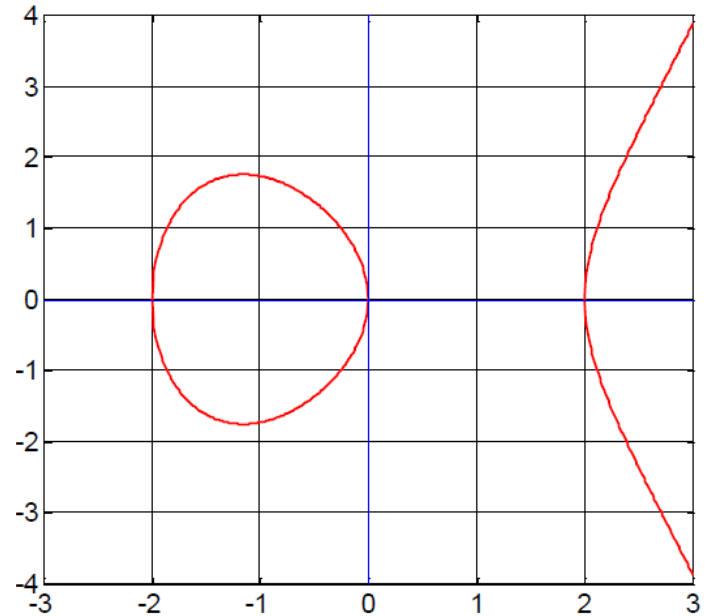
\includegraphics[width=78.12mm,height=169.29mm]{../../images/llm/page_005_img_01.png}%
\end{textblock*}

\end{document}
